\documentclass{beamer}
\usepackage{graphicx}
\usepackage{xcolor}
\usepackage{tikz}
\usepackage{amsmath}

\definecolor{purpleblue}{RGB}{80, 80, 180}
\definecolor{novelPurple}{RGB}{98, 54, 255}
\definecolor{softPurple}{RGB}{180, 170, 255}
\definecolor{softGray}{RGB}{235, 235, 245}
\definecolor{lightText}{RGB}{90, 90, 110}

\usetheme{Madrid}
\usecolortheme{dolphin}
\graphicspath{{static/course_materials/}{static/hard/}{./}}

\setbeamerfont{title}{size=\Large,series=\bfseries}
\setbeamerfont{frametitle}{size=\LARGE,series=\bfseries}
\setbeamercolor{frametitle}{fg=white, bg=novelPurple}
\setbeamercolor{title}{fg=white, bg=purpleblue}

\title[SAT Hard Question 9]{\textbf{SAT Hard Question\\ Set 9}}
\author{\textbf{Jack Zeng}}
\institute{\textcolor{white}{\textbf{Novel Prep}}}
\date{\today}

\begin{document}

\begin{frame}
    \titlepage
    \vfill
    \begin{flushright}
        \textcolor{purpleblue}{\Huge \textbf{Novel Prep}}
    \end{flushright}
\end{frame}

\begin{frame}
    \begin{tikzpicture}[remember picture, overlay]
        \shade[top color=softPurple, bottom color=softGray]
            (current page.north west) rectangle (current page.south east);
        \node[align=center] at (current page.center) {
            {\Huge\bfseries\textcolor{purpleblue}{Novel Prep}} \\[0.5cm]
            {\Large\itshape\textcolor{lightText}{Phase 2 · Hard Question Practice}}
        };
    \end{tikzpicture}
\end{frame}

\begin{frame}{Overview}
    \tableofcontents
\end{frame}

\begin{frame}
\section{Hard Question Set 9}
    \begin{tikzpicture}[remember picture, overlay]
        \shade[top color=softPurple, bottom color=softGray]
            (current page.north west) rectangle (current page.south east);
        \node[align=center] at (current page.center) {
            {\LARGE\bfseries\textcolor{purpleblue}{Hard Question Set 9}} \\[0.5cm]
            {\Large\itshape\textcolor{lightText}{9 SAT-style challenge problems}}
        };
    \end{tikzpicture}
\end{frame}

% --- Question 1 ---
\begin{frame}{Question 1}
\small
Elizabeth has \$4{,}500 in an account. Each year she expects to have \textbf{11\% more} money in the account than the previous year.

Which of the following models best describes how Elizabeth expects the money in her account to change over time?
\vspace{0.35cm}
\begin{enumerate}
    \item[A.] Decreasing exponential
    \item[B.] Decreasing linear
    \item[C.] Increasing exponential
    \item[D.] Increasing linear
\end{enumerate}
\end{frame}
\begin{frame}{Answer 1}
\small
\textbf{Correct Answer:} C
\end{frame}

% --- Question 2 ---
\begin{frame}{Question 2}
\small
The function
\[
T(x) = \frac{20{,}000 - 6.5x}{1{,}000}
\]
gives the estimated air temperature \(T(x)\), in degrees Celsius (\(^\circ\text{C}\)), at an altitude of \(x\) meters.

If the estimated temperature surrounding the hot air balloon is \(15^\circ\text{C}\), which of the following is closest to the altitude \(x\) of the hot air balloon?
\vspace{0.35cm}
\begin{enumerate}
    \item[A.] 20
    \item[B.] 769
    \item[C.] 1,333
    \item[D.] 5,385
\end{enumerate}
\end{frame}
\begin{frame}{Answer 2}
\small
\textbf{Correct Answer:} B
\end{frame}

% --- Question 3 ---
\begin{frame}{Question 3}
\small
The function \(f\) is defined as:
\[
f(x) = (x - a)(x - b)
\]
where \(a\) and \(b\) are integer constants.

Given that:
\[
f(17) > 0,\quad f(20) < 0,\quad f(23) > 0
\]
What is one possible value of \(a + b\)?
\vspace{0.35cm}
\begin{enumerate}
    \item[A.] 39
    \item[B.] 38
    \item[C.] 37
    \item[D.] 36
\end{enumerate}
\end{frame}
\begin{frame}{Answer 3}
\small
\textbf{Correct Answer:} A
\end{frame}

% --- Question 4 ---
\begin{frame}{Question 4}
\small
The positive number \(a\) is 2,106\% of the sum of the positive numbers \(b\) and \(c\), and \(b\) is 81\% of \(c\).

What percent of \(b\) is \(a\)?
\vspace{0.35cm}
\begin{enumerate}
    \item[A.] 4,706\%
    \item[B.] 47.06\%
    \item[C.] 470,600\%
    \item[D.] 47,060\%
\end{enumerate}
\end{frame}
\begin{frame}{Answer 4}
\small
\textbf{Correct Answer:} A
\end{frame}

% --- Question 5 ---
\begin{frame}{Question 5}
\small
For the function \(f\), for every increase of 2 in the value of \(x\), the value of \(f(x)\) increases by a factor of \(c\), where \(c\) is a constant.

Which of the following equivalent forms of function \(f\) displays the value of \(c\) as the base or the coefficient?
\vspace{0.35cm}
\begin{enumerate}
    \item[A.] \(f(x) = 42(2)^{6x}\)
    \item[B.] \(f(x) = 42(8)^{2x}\)
    \item[C.] \(f(x) = 42(64)^x\)
    \item[D.] \(f(x) = 42(4096)^{x/2}\)
\end{enumerate}
\end{frame}
\begin{frame}{Answer 5}
\small
\textbf{Correct Answer:} D
\end{frame}

% --- Question 6 ---
\begin{frame}{Question 6}
\small
A study investigated the effect of magnesium supplementation on sleep quality. 190 adults were randomly selected, and their sleep efficiency was measured.

Participants were randomly assigned to take a magnesium supplement or a placebo for 6 weeks. The study concluded that magnesium improved sleep quality.

What feature of this study supports this conclusion?
\vspace{0.35cm}
\begin{enumerate}
    \item[A.] There were more than 100 participants in the study.
    \item[B.] The participants were selected at random from the community center.
    \item[C.] The sleep efficiency of each participant was measured again at the end of 6 weeks.
    \item[D.] Each participant was randomly assigned to take a magnesium supplement or a placebo.
\end{enumerate}
\end{frame}
\begin{frame}{Answer 6}
\small
\textbf{Correct Answer:} D
\end{frame}

% --- Question 7 ---
\begin{frame}{Question 7}
\small
A circle in the \(xy\)-plane has its center at \((-1, 1)\). Line \(t\) is tangent to this circle at the point \((7, -6)\).

Which of the following points also lies on line \(t\)?
\vspace{0.35cm}
\begin{enumerate}
    \item[A.] \((0, 7)\)
    \item[B.] \((6, 9)\)
    \item[C.] \((14, 2)\)
    \item[D.] \((15, 1)\)
\end{enumerate}
\end{frame}
\begin{frame}{Answer 7}
\small
\textbf{Correct Answer:} C
\end{frame}

% --- Question 8 ---
\begin{frame}{Question 8}
\small
The function \(f(x)\) is defined by:
\[
f(x) = \frac{x^2 + ax + b}{2x + c}
\]
where \(a\), \(b\), and \(c\) are constants.

The graph of \(f(x)\) does not intersect the line \(x = 4\). If \(f(5) = f(6) = 0\), what is the value of \(a + b + c\)?
\vspace{0.35cm}
\begin{enumerate}
    \item[A.] 10
    \item[B.] 11
    \item[C.] 12
    \item[D.] 13
\end{enumerate}
\end{frame}
\begin{frame}{Answer 8}
\small
\textbf{Correct Answer:} B
\end{frame}

% --- Question 9 ---
\begin{frame}{Question 9}
\small
\begin{center}
    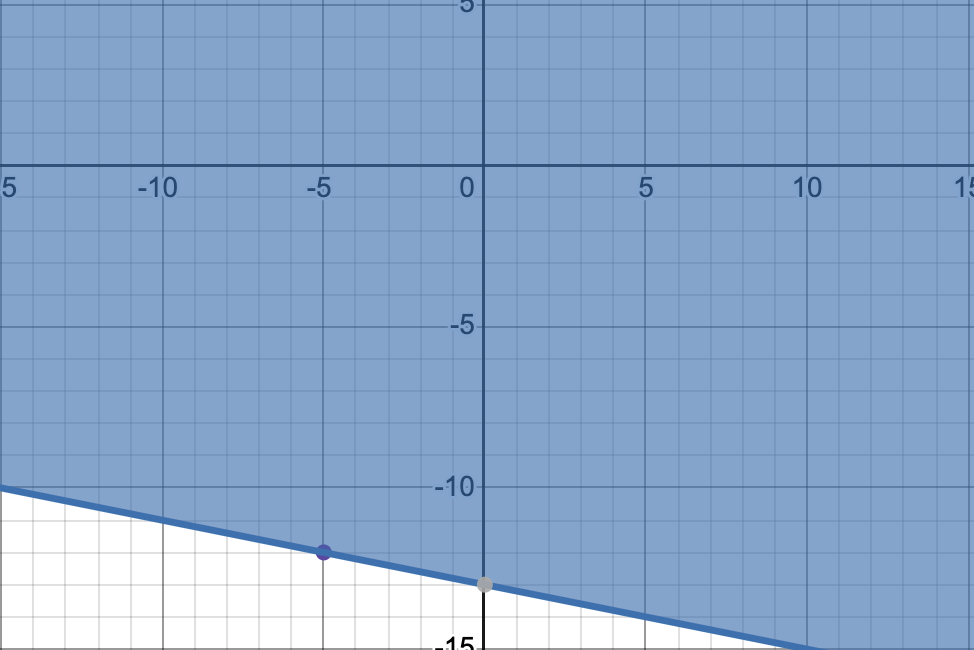
\includegraphics[width=0.42\linewidth]{hard_9_f7.png}
\end{center}

The shaded region represents the solutions to the inequality:
\[
rx + ty \geq -65
\]
What is the value of \(r + t\)?
\vspace{0.35cm}
\begin{enumerate}
    \item[A.] 6
    \item[B.] 4
    \item[C.] -4
    \item[D.] -5
\end{enumerate}
\end{frame}
\begin{frame}{Answer 9}
\small
\textbf{Correct Answer:} A
\end{frame}

\begin{frame}{}
    \begin{tikzpicture}[remember picture, overlay]
        \shade[top color=novelPurple!40, bottom color=white]
            (current page.north west) rectangle (current page.south east);
        \fill[white, opacity=0.15] (current page.center) circle (5cm);
        \foreach \x in {1,2,3,4,5} {
            \fill[novelPurple, opacity=0.12] (rand*10-5, rand*7-3.5) circle (0.1+\x*0.05);
        }
    \end{tikzpicture}
    \centering
    \vspace{5em}
    {\Huge \textbf{\textcolor{novelPurple}{Thank You!}}} \\[1em]
    {\large \textcolor{gray}{We appreciate your time and focus.}} \\[3em]
    {\LARGE \textbf{\textcolor{novelPurple}{\textsf{Novel Prep}}}}
    \vfill
\end{frame}

\end{document}
